\documentclass[12pt]{article}
\usepackage{float}
\usepackage{caption}
\usepackage{times}
\usepackage{natbib}
\usepackage{graphicx}
\usepackage[section]{placeins}
\usepackage{indentfirst}
\usepackage{fancyhdr}
\usepackage{xcolor}

\usepackage{listings}
\usepackage{color}
\usepackage[hyphens,spaces,obeyspaces]{url}
\usepackage{hyperref}
\pagenumbering{roman}
\hypersetup{
    colorlinks=true,
    linkcolor=black,
    urlcolor=black,
    citecolor = gray,
    linktoc=all
}
\lstset{language=C,
    basicstyle=\ttfamily,
    keywordstyle=\bfseries,
    showstringspaces=false,
    morekeywords={include, printf,transactionManager,transaction,startTransaction,TM, TX,createTX,destroyTX,storeTransaction,commitTransaction,commitTransactions,std::this_thread::get_id()}
}
\lstset { %
	language=C++,
	backgroundcolor=\color{black!5}, % set backgroundcolor
	basicstyle=\footnotesize,% basic font setting
}
\pagestyle{fancy}
\fancyhf{}
\rhead{\textit{\color{gray}\today}}
\lhead{\textit{\color{gray}C++14 Software Transactional Memory}}
\rfoot{Page \thepage}
\lfoot{\color{gray}\LaTeX}

\pagenumbering{roman}
\begin{document}

\begin{titlepage}
	\begin{center}
	\line(1,0){350}\\
	[0.3 cm]
	\huge{\textbf{Software Transactional Memory\\[0.3 cm]C++14 STM\\ }} 
	\line(1,0){200}\\
	[0.3 cm]
	\huge{\textbf{Design manual }} 
		\begin{LARGE}
		\\[0.3 cm]Zoltan Fuzesi\\
		\today
		\end{LARGE}
		
		\begin{LARGE}
		\line(1,0){150}\\
		[1.0 cm]
		Student ID: C00197361\\
		Supervisor: Joseph Kehoe\\
		\color{gray}Institute of Technology Carlow\\
		\color{gray}Software Engineering
		\end{LARGE}
		
\begin{figure}[h!]
\centering

\includegraphics[scale=0.7]{Pictures/carlow.png}
\end{figure}
		
	\end{center}
\end{titlepage}

\tableofcontents







\clearpage
\pagenumbering{arabic}
\setcounter{page}{1}

\section{Introduction}
This document is introducing the design of the C++ STM library logic and structure. The document will describe the flow of the data within the library and the external application that uses the STM library. The use case diagram will discover the possible library API interface functionalities that need to implement in the project. With the use cases and the detailed use cases can characterize the required steps and potential alternative steps during the library execution life cycle. The domain model shows the main functionality of the library and the association between the software components, follows with the sequence diagram that helps to understand the sequence of steps required to implement lock free, object based locking, transactional mechanism.\\

This document helps to discover the potential errors and required handlers with the use cases and the sequence diagram. However, this diagrams and use case descriptions are identify the potential issues and risks, that may can mislead the future development if not well designed. To use, or test the STM library implementation, the programmers must to write their own client application and includes the library, like any other (external) libraries in C or C++ programming design. The usage of the library will happen with the API function calls, that will be described in the use case diagram and studies thoroughly in the detailed use cases.\\
 
 
\newpage
\section{Model of the application}
The flow diagram \textit{Figure 2} introducing the dynamic relationship of the STM library. This relations interacting with the client application and the objects delegated by the STM library. In order to use the STM library, the programmers must include it in the main module, to create an instance of a transaction manager, associated with the application by the Process ID to use the API interfaces. When the instances is created then the API function will be available to the client application. The key of the library usage, the connected processes can not instantiate more then one transaction manager object of the library, because the library use singleton object instantiation, that keep track of all process accessed the transaction manager by the process ID. This way the library can register all connected process in the built in Data structure.

\subsection{Library integration to the client application}
The final solution will include shared and static library solution. The shared library is linked to the client application at compilation time, and the code can be shared between multiple processes. The static library code gets integrated to the client application, which is not shared with other processes. With the booth solution the header files must used as a reference to the library API functions. When the executable created, the header files and the static library file are not required any more. The shared library should be kept somewhere in the operating system.\\


\begin{figure}[h!]
\centering
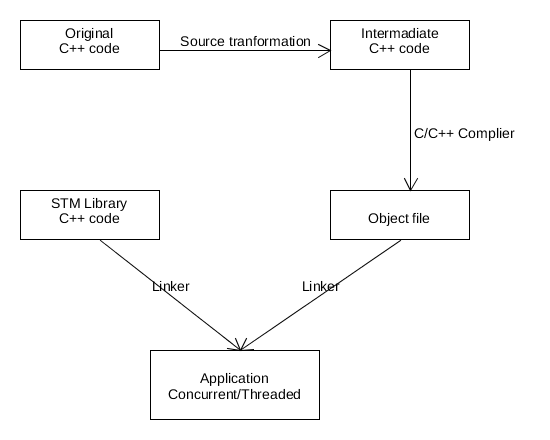
\includegraphics[scale=0.5]{Pictures/transformation.png}
\caption{\textit{\color{gray}STM library linked to application.}}
\end{figure}

\newpage
\subsection{Flow diagram}
\begin{figure}[h!]
\centering
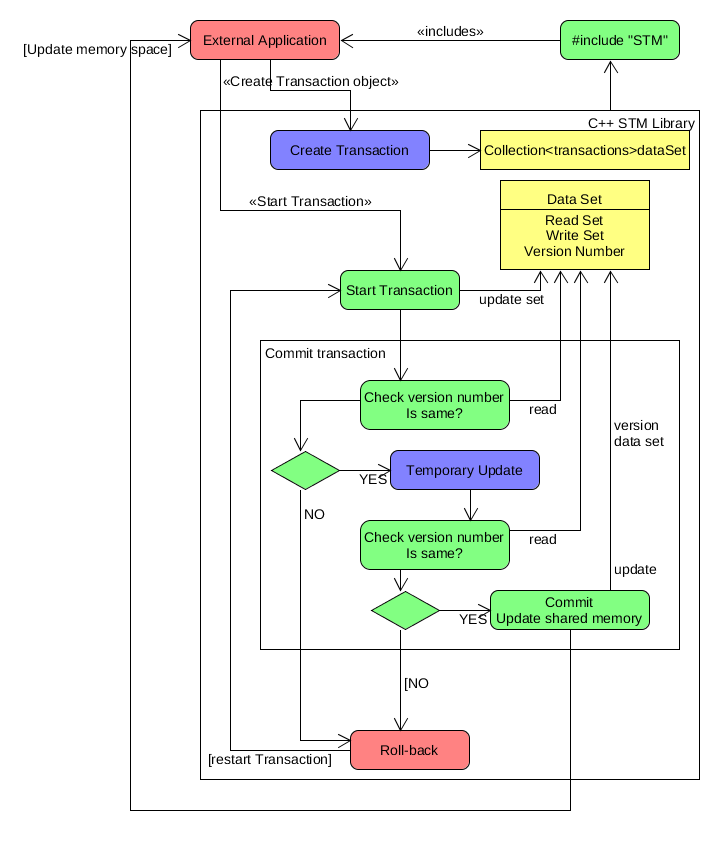
\includegraphics[scale=0.5]{Pictures/flowDiagram.png}
\caption{\textit{\color{gray}The flow of the data in the library.}}
\end{figure}

When the \textbf{create transaction} API call happens by the application, the library place a new transactional object into the built in data structure, associating by the process ID and returning back a transactional object to the given application.\\

The \textbf{start transaction} API call will starting the process of the Object transactional life cycle. First, place the object into the (global shared) read set, and creates a copy of it to the write set, to use it for local temporary changes, and add a version number to it, as a counter to determine the Object changes. Because more then one thread can use the same object, it must check the version number at the first step to determine the changes at early stage of the object transactional life cycle. If the version number in the object is different then the global version number, the transaction will cancel and restart. If the version number that the object hold and the global version number in the write set are same, then the copy of the object in the write set will update to the new required value. Before the original object can change from the local copy, the transaction library must check the version numbers equality again. If the version numbers are same, that means no other process accessed the same object during the updating process, and the object can get assign the new value. Otherwise, the transaction must cancel and the life cycle restart again.\\

In this phase of the program execution, the transaction marked as processable process, and the \textbf{commit method} available for execution. This API call will update the original object, update/increase the version number assigned to it and returns back to the main process to finish its execution. If other processes or thread are still using the same object, they must detect the changes on the version number, and restart the transaction if required.

\newpage
\section{API usage}
This part of the document will design the library API interface function(s), that will use by the external application. First, the library function (API) calls will be demonstrated with a simple test application, then the library methods.\\

\begin{lstlisting}[
    basicstyle=\tiny, %or \small or \footnotesize etc.
]
#include <STM.h>
#include <sstream> //get the thread id
#include <unistd.h> //get the Application process id

//Create a Transaction manager
TM transactionManager;
//Create a transaction object
TX transaction;

class Account : public Tobj{
	private:
			int amount;
			int accountID;
			string accountHolder;
			Account(int amount, int accountID, string accountHolder):Tobj(){
				this->amount = amount;
				this->accountID = accountID;
				this->accountHolder = accountHolder;
			}
	public:
		void addAmount(double amount){
			this->amount += amount;
		}

		void removeAmount(double amount){
			this->amount -= amount;
		}
		double getAmount(){
			return this->amount;
		}
		int getAccountId(){
			return accountID;
		}

}

//Single object operation
bool updateAccount(std::shared_ptr<Account> account, double amount){

	//All threads updating account * times
	for(int i = 0; i < updateTimes; ++i)
		{

	
			Account tmp = loadTransactionObject(std::this_thread::get_id());
			tmp.addAmount(*amount);

			transaction.storeTransaction(std::this_thread::get_id(), &tmp);
		}

		barrier->Wait();
		bool done = false
		//All threads commits their transactions
		while(!done){
			Account tmp = loadTransactionObject(std::this_thread::get_id());
			done = transaction.commitTransaction(std::this_thread::get_id(), &tmp);
		}
		barrier->Start();

	return true; 
}


//multiple objects operations
bool exchange(double amount, std::vector<Account>*acconts){
	
	//Create boolean value to check the transaction state
 	bool done = false;

 	while(!done){
 		//make changes on the copy of the objects
  		acconts[0].addAmount(amount);
  		acconts[1].removeAmount(amount);

  		//The transaction updates the local copy of the object in the library
  		transaction.storeTransaction(std::this_thread::get_id(), &acconts);

 		//The transaction try to update the values in the transaction
 		//if the values update then return true otherwise return false
 		done = transaction.commitTransactions(*accounts);
  	}
  	return true;
}

int main(){
	 //get the process id
	 pid_t ppid;
     ppid = getppid();
	 //create a thread
	 std::thread threadOne;
	 //Create shared poinetrs of the bank accounts
	 std::shared_ptr<Account> from(100,1234,"JOE");
	 std::shared_ptr<Account> to(50,2345,"BOB");

 	//add the thread to the TM manager HasMap and return the transaction
 	transaction = transactionManager.createTX(ppid);

 	//transaction add the account object to the transaction HasMap read and write sets and return the local copy 
 	auto copyFrom = transaction.startTransaction(std::this_thread::get_id(), &from);
	auto copyTo = transaction.startTransaction(std::this_thread::get_id(), &to);

	//Add the local copies to the vector to store all the associated transactions
	std::vector<Accont*> accounts;
	accounts.push_back(copyFrom);
	accounts.push_back(copyTo);

	//Amount to work with
	double amountToExchange = 100.5;

	//Thread call the function and passing all the required variables to operate the transaction
	threadOne=std::thread(exchange, copyFrom, copyTo, amountToExchange, &accounts);
 	
	//create a thread
	 std::thread threadTwo, threadThree, threadFour, threadFive, threadSix;

	 //All the threads are calling the same function with the same object to make changes
	 threadTwo   = std::thread(updateAccount, copyFrom, 1, 5);
	 threadThree = std::thread(updateAccount, copyFrom, 1, 5);
	 threadFour  = std::thread(updateAccount, copyFrom, 1, 5);
	 threadFive  = std::thread(updateAccount, copyFrom, 1, 5);
	 threadSix   = std::thread(updateAccount, copyFrom, 1, 5);


	threadOne.join();
	threadTwo.join();
	threadThree.join();
	threadFour.join();
	threadFive.join();
	threadSix.join();



	//Otherwise destroy the manager that clean out the memory from
	//all the transactions
	transactionManager.destroy(ppid);
	
	return 0;
}

\end{lstlisting}

\newpage
\subsection{Create transaction}
\begin{lstlisting}[
    basicstyle=\tiny, %or \small or \footnotesize etc.
]
//Create transaction associated with Application
TX createTX(pid_t ppid){

	MAP::const_iterator position = transactions.find(ppid);
	TX tx;
	if (position == map.end()) {
	    tx = new TX();
		transactions[ppid] = tx;
	} 

	retrun Tx;
}
\end{lstlisting}

\subsection{Destroy transaction}
\begin{lstlisting}[
    basicstyle=\tiny, %or \small or \footnotesize etc.
]
//Destroy transaction associated with Application
bool destroyTX(pid_t ppid){

	MAP::const_iterator position = transactions.find(id);
	if (position == map.end()) {
	    return true
	}else{
		transactions[ppid] = null;
	}

	return true;
	
}
\end{lstlisting}

\subsection{Start transaction}
\begin{lstlisting}[
    basicstyle=\tiny, %or \small or \footnotesize etc.
]
//store object in read and write set
bool startTransaction(std::thread::id id, Tobj* obj){

	MAP::const_iterator position = readSet.find(id);
	//Update data set only if not registered
	if (position == map.end()) {
		obj.setVersionNumber(0);
	    //register object to the read set
		readSet[id] = boj;
		//Call the copy constructor to make a copy of the object
		Tobj objCopy = obj;
		objCopy.setVersionNumber(0);
		//Register object to the write set as a copy of the original
		Tobj object = copyObject(obj)
		writeSet[id] = object;
	} 
	
	return true;
}
\end{lstlisting}


\subsection{Commit transaction}
\begin{lstlisting}[
    basicstyle=\tiny, %or \small or \footnotesize etc.
]
//Commit Transaction , single object transaction
bool commitTransaction(std::thread::id id, Tobj* obj){
	//Compare the working write set object version number with the read set version number
	if(obj.getVersionNumber() == getVersionNumber(id)){
		//Update write set object values
		updateTransaction(*obj);
		//before change the readset checks again for version number
		if(obj.getVersionNumber() == getVersionNumber(id)){
			updateSharedMemory(*obj);
			obj.incrementVersionNumber();
			return true;
		}else{
			rollbackTransaction(id);
			return false;
		}
	}
	//If not same return false and restart
	return false;
}
\end{lstlisting}

\subsection{Commit transactions}
\begin{lstlisting}[
    basicstyle=\tiny, %or \small or \footnotesize etc.
]
//Commit Transactions , multiple objects transactions
bool commitTransactions(std::thread::id id, vector<Tobj*> & accounts){
	 for (int i=0; i<accounts.size(); i++)
    {
    		//get the object
    		Tobj* obj = getObject(id);
        if(accounts[i].getVersionNumber())  == obj.getVersioNumber(){
        	//Update write set object values
			updateTransaction(*obj);
			if(accounts[i].getVersionNumber())  == obj.getVersioNumber(){
				updateSharedMemory(*accounts[i]);
				*accounts[i].incrementVersionNumber();
				//If all object has updated
				if(i == accounts.size()-1){
					return true;
				}
			}else{
				rollbackTransaction(id);
				return false;
			}
    	}
    }	

		

	return false;
}

\end{lstlisting}



\subsection{Load Transaction Object}
\begin{lstlisting}[
    basicstyle=\tiny, %or \small or \footnotesize etc.
]
//Load transaction return object
Tobj* loadTransactionObject(std::thread::id id, Tobj* obj){

	return &writeSet[id];
}
\end{lstlisting}

\subsection{Store transaction}
\begin{lstlisting}[
    basicstyle=\tiny, %or \small or \footnotesize etc.
]
//Store transaction is updating the object in the write set 
bool storeTransaction(std::thread::id id, Tobj* obj){
		//Update/overwrite collection value by  
		writeSet[id] = obj;
	
	return true;
}
\end{lstlisting}

\subsection{Store transactions}
\begin{lstlisting}[
    basicstyle=\tiny, %or \small or \footnotesize etc.
]
//Store transaction is updating the object in the write set 
bool storeTransactions(std::thread::id id, vector<Tobj*> & accounts){
	//Update/overwrite collection value by  
        writeSet[id] = accounts;

	return true;
}
\end{lstlisting}

\newpage
\section{Use case}
This section of the document the use case diagram will list the API functions or events, to define the interactions between the client application and the library.

\begin{figure}[h!]
\centering
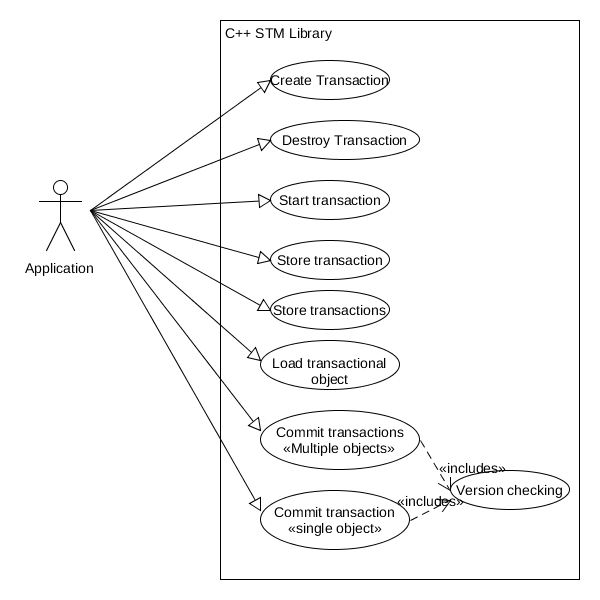
\includegraphics[scale=0.35]{Pictures/usecase.png}
\caption{\textit{\color{gray}The STM library API actions.}}
\end{figure}
{\setlength{\parindent}{0cm}
\subsection{Brief case}
\subsubsection{Create transaction}
\textbf{Use case} : Create transaction.\\
\textbf{Actors} : Application\\
\textbf{Description} : This use case begin when Application wants instantiate an object of the STM transactional library. The library registering a new transactional object by the process Id and returning the transactional object that can use the library API interface, which ends this use case.\\
\subsubsection{Destroy transaction}
\textbf{Use case} : Destroy transaction.\\
\textbf{Actors} : Application\\
\textbf{Description} : This use case begin when Application wants to destroy the object of the STM transactional library associated with the application. The application calls the API function and send the process Id, that is deleting the object from the data set, which ends this use case.\\
\subsubsection{Start transaction}
\textbf{Use case} : Start transaction.\\\
\textbf{Actors} : Application\\
\textbf{Description} : This use case begin when Application wants to add a new object to the STM library. The transactional object call the API function and send the Object and the thread id which wants to operate on it. This object will be registered in the library read data set and a copy of it in the write data set, which ends this use case.\\  
\subsubsection{Start transactions}
\textbf{Use case} : Start transactions.\\\
\textbf{Actors} : Application\\
\textbf{Description} : This use case begin when Application wants to add new objects to the STM library. The transactional object call the API function and send the collection of Objects with the thread id  which wants to operate on it. This objects will be registered in the library read data set and a copy of it in the write data set, which ends this use case.\\ 
\subsubsection{Commit transaction}
\textbf{Use case} : Commit transaction.\\
\textbf{Actors} : Application\\
\textbf{Description} : This use case begin when Application wants commit or make permanent changes on the object shared value, while that is not available to the other processes. The transactional object calls the commit transaction function call. The library checking the version number associated with the thread ant the object. If the version numbers are same in the global data set and the object itself, then the STM library updates the read set and checks the write set again to the version number. If the version number is still the same, then the library updates the shared memory space permanently and indicate the application that the object have been updated, which ends this use case.\\ 
\subsubsection{commit transactions}
\textbf{Use case} : Commit transactions.\\
\textbf{Actors} : Application\\
\textbf{Description} : This use case begin when Application wants commit or make permanent changes on more objects shared value, while those are not available to the other processes. The transactional object calls the commit transaction function call. The library goes through on all the objects in the collection set, and doing the following process on each object.First checking the version number associated with the object. If the version numbers are same in the global data set and the object itself, then the STM library updates the write set and checks the read set again to the version number. If the version number is still the same, then the library updates the shared memory space permanently and indicate the application that the object have been updated,  which ends this use case.\\
\subsubsection{Load Transaction object}
\textbf{Use case} : Load Transaction object.\\
\textbf{Actors} : Application\\
\textbf{Description} : This use case begin when Application wants to receive the copy of the object from the STM library. The application calls the API function and passing the thread Id, that is returning back the copy of the object associated with the thread Id, which ends this use case.\\
\subsubsection{Store transaction}
\textbf{Use case} : Store transaction.\\
\textbf{Actors} : Application\\
\textbf{Description} : This use case begin when Application wants to store an object involved in the transaction. The transaction object calls the store transaction API function, that will save the object associated with the thread id, which ends this use case.\\
\subsubsection{Store transactions}
\textbf{Use case} : Store transactions.\\
\textbf{Actors} : Application\\
\textbf{Description} : This use case begin when Application wants to store more object involved in the transaction. The transaction object calls the store transactions API function, that will goes through on the object  collection and save all the objects associated with the thread id, which ends this use case.\\
}
\newpage
\subsection{Detailed use case}
{\setlength{\parindent}{0cm}
\subsubsection{Create transaction}
\textbf{Name} : Create transaction.\\
\textbf{Actors} : Application\\
\textbf{Main Scenario.}
\begin{enumerate}
  \item The use case begins when the Application wants to create a transactional object.
  \item The Application calls the create transaction function in the transaction manager.
  \item The library check for the existence of the transaction.
  \item The library returns the transactional object to the Application.
\end{enumerate}
\textbf{Alternatives}\\
4a. The transaction is not exist the library need to create.\\

\begin{figure}[h!]
\centering
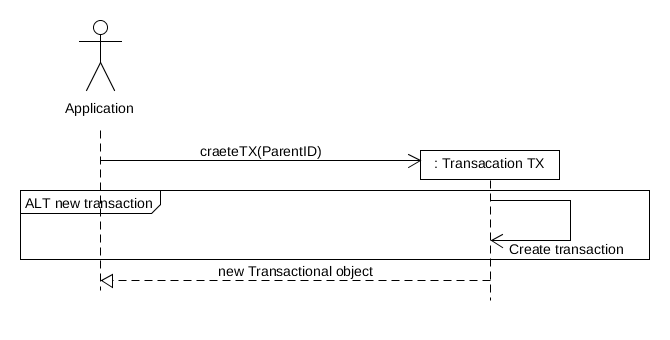
\includegraphics[scale=0.4]{Pictures/create.png}
\caption{\textit{\color{gray}Create transaction.}}
\end{figure}


\subsubsection{Destroy transaction}
\textbf{Name} : Destroy transaction.\\
\textbf{Actors} : Application\\
\textbf{Main Scenario.}
\begin{enumerate}
  \item The use case begins when the Application wants to destroy the transaction object.
  \item The Application calls the destroy transaction function in the transaction manager.
  \item The library check for the existence of the transaction.
  \item The library delete the transaction  
  \item The library returns the transactional object to the Application.
\end{enumerate}


\begin{figure}[h!]
\centering
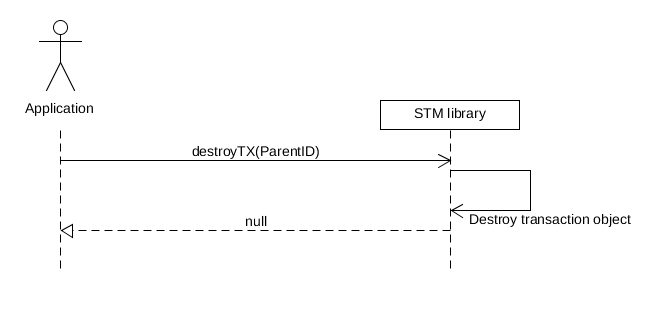
\includegraphics[scale=0.5]{Pictures/destroy.png}
\caption{\textit{\color{gray}Destroying transaction object.}}
\end{figure}

\subsubsection{Start transaction}
\textbf{Name} : Start transaction.\\
\textbf{Actors} : Application\\
\textbf{Main Scenario.}
\begin{enumerate}
  \item The use case begins when Application wants add an object to the transactional library.
  \item The Application call the start transaction API function and passing the object and thread Id to the library.
  \item The library registering the object to the read data set and creates a copy of it to the write data set.
  \item The library assign a version number to the registered object.
  \item The library indicate the Application that the object registered with the returned copy of it.
\end{enumerate}
\textbf{Alternatives}\\
3a. The object already in the data set don't need to be register.\\

\begin{figure}[h!]
\centering
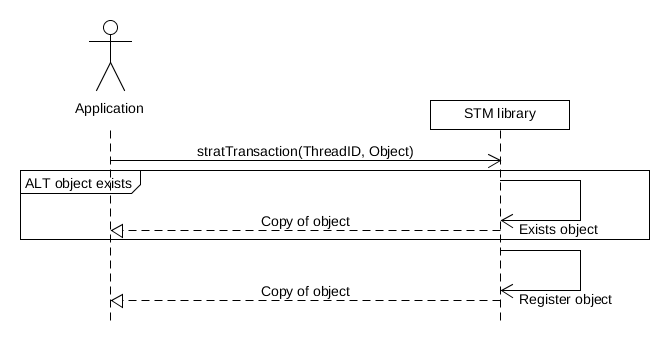
\includegraphics[scale=0.5]{Pictures/start.png}
\caption{\textit{\color{gray}Start transaction.}}
\end{figure}

\subsubsection{Start transactions}
\textbf{Name} : Start transactions.\\
\textbf{Actors} : Application\\
\textbf{Main Scenario.}
\begin{enumerate}
  \item The use case begins when Application wants add collection of objects to the transactional library.
  \item The Application call the start transaction API function and passing the object collection to the library.
  \item The library goes through on the collection and registering each objects to the read data set and creates  a copy of it to the write data set.
  \item The library assign a version number to each registered objects.
  \item The library indicate the Application that the object registered with the returned copy of the collection of objects.
\end{enumerate}
\textbf{Alternatives}\\
3a. The objects already in the data set don't need to be register.\\

\begin{figure}[h!]
\centering
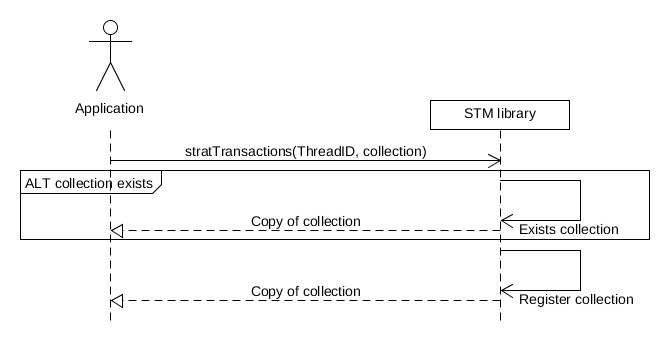
\includegraphics[scale=0.5]{Pictures/startTransactions.png}
\caption{\textit{\color{gray}Start transactions.}}
\end{figure}

\subsubsection{Commit transaction}
\textbf{Name} : Commit transaction.\\
\textbf{Actors} : Application\\
\textbf{Main Scenario.}
\begin{enumerate}
  \item The use case begins when the Application wants to make the changes on the object value.
  \item The Application calls the commit transaction function call on the API and passing the required values to exchange within the object.
  \item The library checks the version number associated with the object.
  \item The library make changes on the copy of the object in the local data set.
  \item The library checks again the version number associated with the object. 
  \item The library make the permanent change on the object.
  \item The library indicates the Application that the changes has made with the true boolean answer.
\end{enumerate}
\textbf{Alternatives}\\
3a. The library early find the difference between the version numbers.\\
3b. The library cancel the transaction and indicates the Application with a false answer.\\
5a. The library later stage find the difference between the version numbers.\\
5b. The library cancel the transaction and indicates the Application with a false answer.\\

\begin{figure}[h!]
\centering
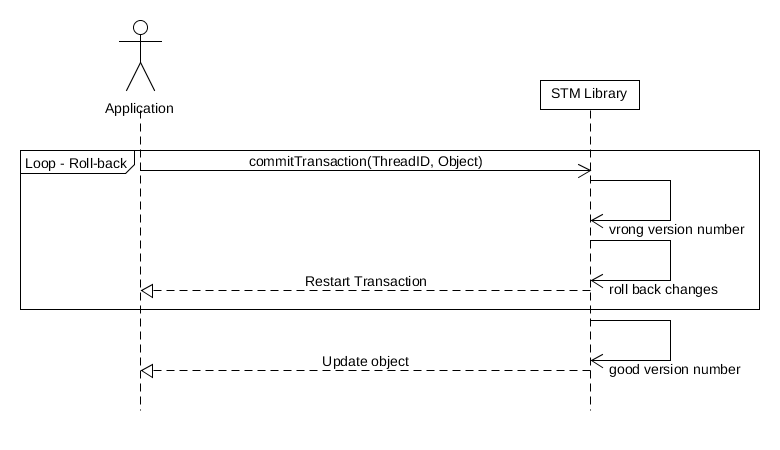
\includegraphics[scale=0.5]{Pictures/commit.png}
\caption{\textit{\color{gray}Commit transaction.}}
\end{figure}

\subsubsection{Commit transactions}
\textbf{Name} : Commit transactions.\\
\textbf{Actors} : Application\\
\textbf{Main Scenario.}
\begin{enumerate}
  \item The use case begins when the Application wants to make the changes on collection of object values.
  \item The Application calls the commit transaction function call on the API and passing the required collection to exchange within the objects.
  \item The library goes through every single object.
  \item The library checks the version number associated with the object.
  \item The library make changes on the copy of the object in the local data set.
  \item The library checks again the version number associated with the object. 
  \item The library make the permanent change on the object.
  \item The library indicates the Application that the changes has made with the true boolean answer.
\end{enumerate}
\textbf{Alternatives}\\
3a. The library early find the difference between the version numbers.\\
3b. The library cancel all the transaction and indicates the Application with a false answer.\\
5a. The library later stage find the difference between the version numbers.\\
5b. The library cancel all the transaction and indicates the Application with a false answer.\\

\begin{figure}[h!]
\centering
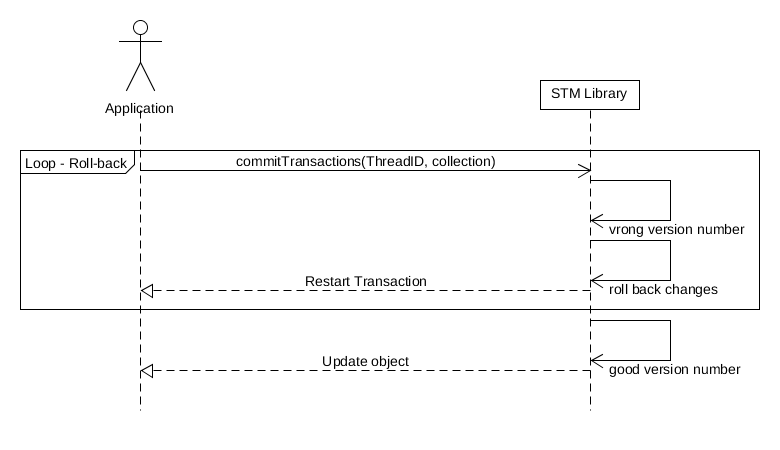
\includegraphics[scale=0.3]{Pictures/commitTransactions.png}
\caption{\textit{\color{gray}Commit transactions.}}
\end{figure}

\newpage
\subsubsection{Load transaction}
\textbf{Name} : Load transaction.\\
\textbf{Actors} : Application\\
\textbf{Main Scenario.}
\begin{enumerate}
  \item The use case begins when the Application wants receive a copy of an object.
  \item The Application calls the load transaction object function in the library API. 
  \item The library returning back the object determined by the id. 
\end{enumerate}
\textbf{Alternatives}\\
3a. The library can not find the Object by the id..\\

\begin{figure}[h!]
\centering
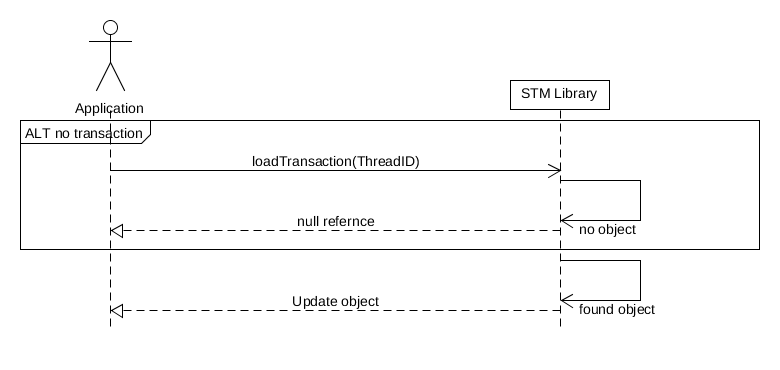
\includegraphics[scale=0.5]{Pictures/load.png}
\caption{\textit{\color{gray}Receive back object from transaction.}}
\end{figure}

\subsubsection{Store transaction}
\textbf{Name} : Store transaction.\\
\textbf{Actors} : Application\\
\textbf{Main Scenario.}
\begin{enumerate}
  \item The use case begins when the Application wants to register a single object in the library.
  \item The Application calls the store function and sending the object and the thread id to the library API interface.
  \item The library registering the object by the id.
\end{enumerate}
\textbf{Alternatives}\\
3a. The object is null equivalent.\\

\begin{figure}[h!]
\centering
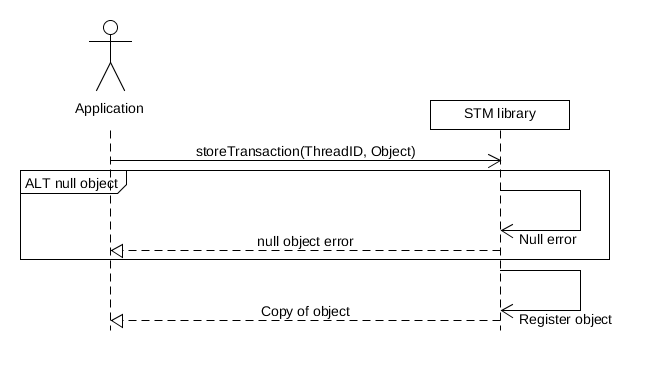
\includegraphics[scale=0.5]{Pictures/store.png}
\caption{\textit{\color{gray}Add object to transaction.}}
\end{figure}

\subsubsection{Store transactions}
\textbf{Name} : Store transactions.\\
\textbf{Actors} : Application\\
\textbf{Main Scenario.}
\begin{enumerate}
  \item The use case begins when the Application wants register a collection of objects.
 \item The Application calls the store function and sending the object collection to the library API interface.
  \item The library goes  through and registering each objects by the id.
\end{enumerate}
\textbf{Alternatives}\\
3a. The collection contains null equivalent object.\\

\begin{figure}[h!]
\centering
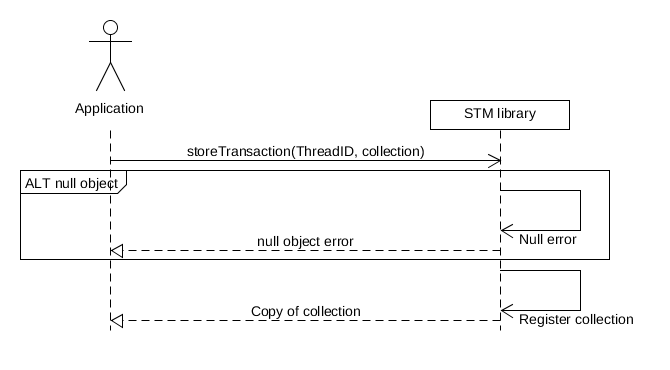
\includegraphics[scale=0.5]{Pictures/storeTransactions.png}
\caption{\textit{\color{gray}Add collection to the transaction.}}
\end{figure}

}

\newpage
\section{System sequence diagram}
\begin{figure}[h!]
\centering
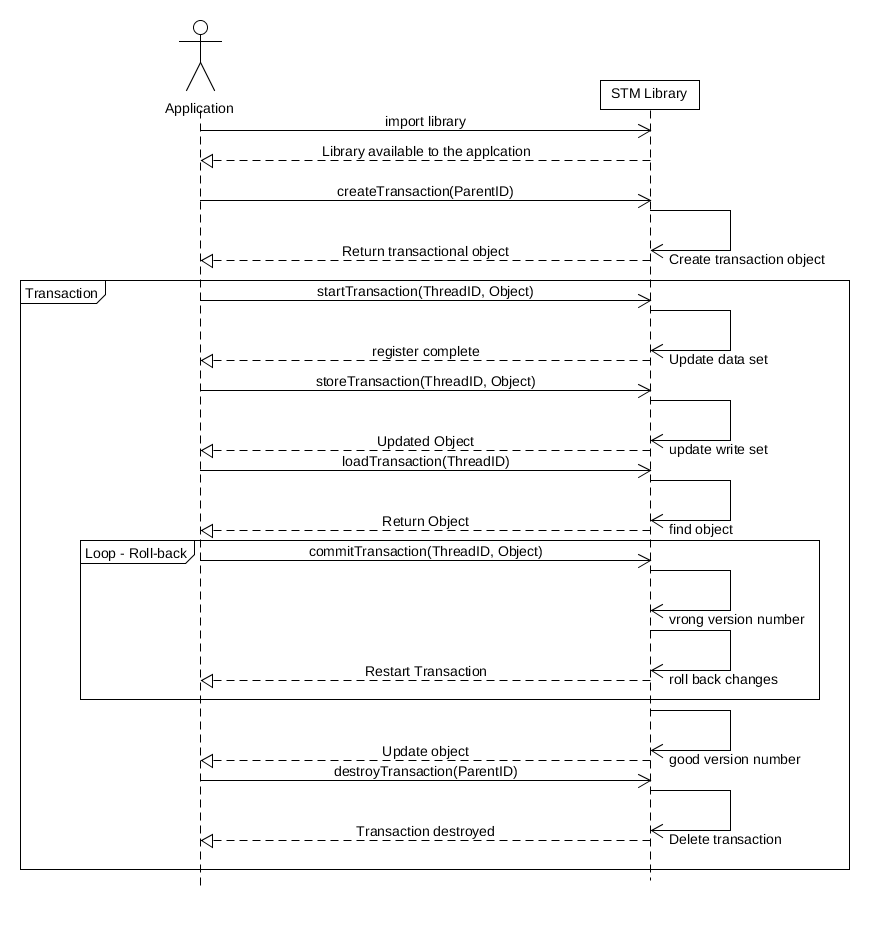
\includegraphics[scale=0.45]{Pictures/sequence.png}
\caption{\textit{\color{gray}The system sequence diagram.}}
\end{figure}

\newpage
\section{Domain model}
The domain model is quiet simple since the library do not need include many classes and functions to implement the Software Transactional Memory implementation with the basic functions. Of course, many STM library has implementation of different binary trees as well, that make it more bigger and complex. 
\begin{figure}[h!]
\centering
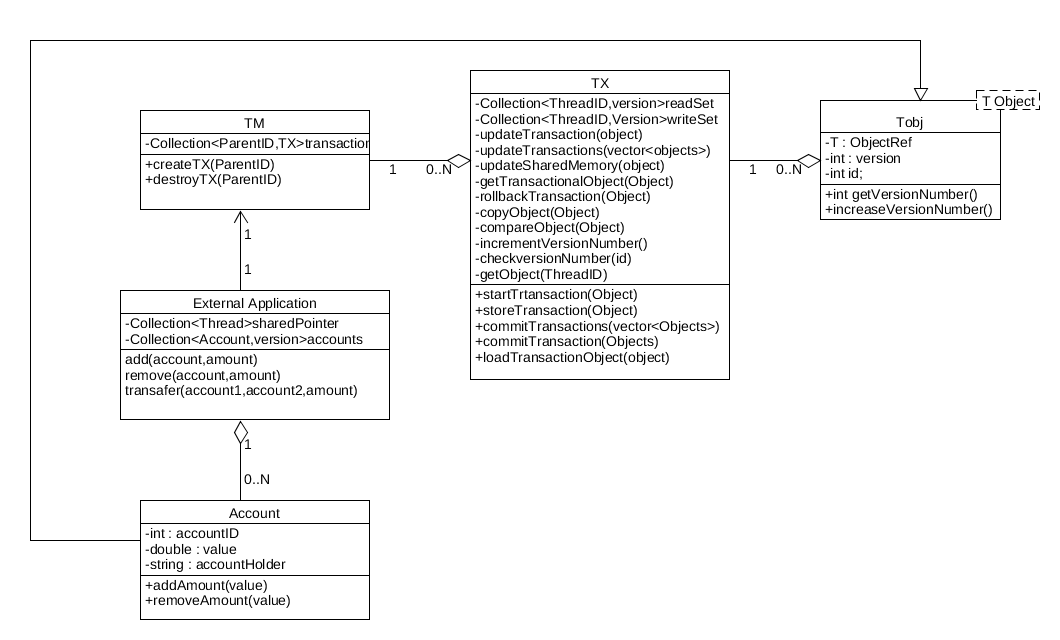
\includegraphics[scale=0.25]{Pictures/domainModel.png}
\caption{\textit{\color{gray}The class hierarchy.}}
\end{figure}

\begin{figure}[h!]
\centering
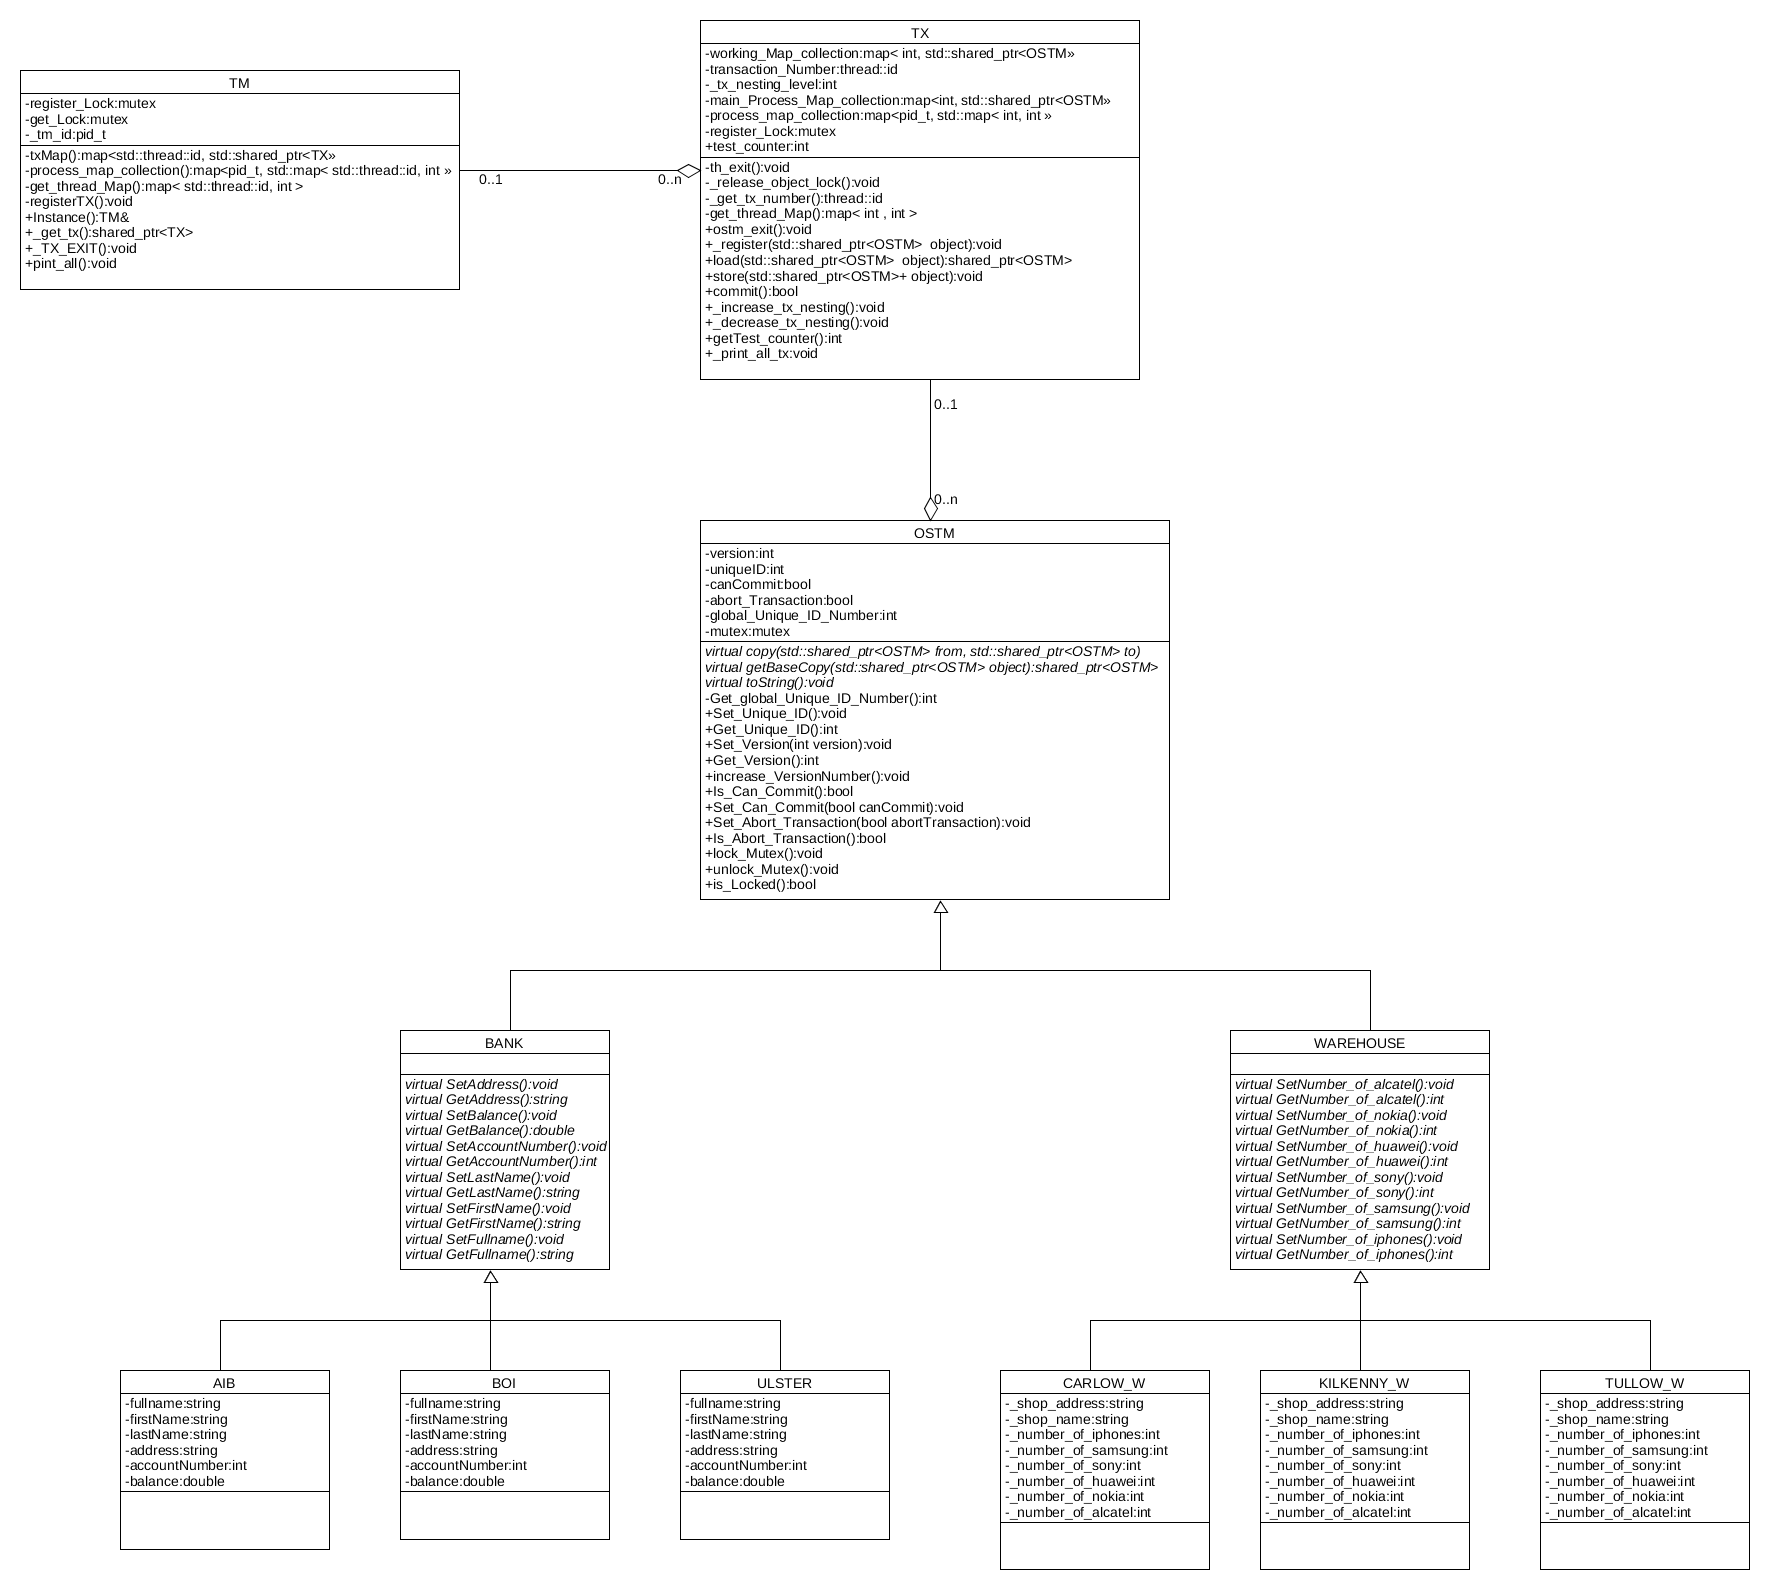
\includegraphics[scale=0.25]{Pictures/Domain_model.png}
\caption{\textit{\color{gray}Updated Domain Model.}}
\end{figure}

\section{Testing the STM Library}
One way to test the Software Transaction Memory library functionalities, is to create a client application and include the shared library in it. The other way is to use a C++ Testing framework such as CppUnit to test API functions and the library itself.
As the library getting more functionality during the development, those functions should be tested one by one. Because the functions have return values, it makes the testing process more easier.\\

\textbf{The functions can be tested separately like:}
\begin{enumerate}
\item The library available from the test application.
\item The library can be instantiated by the application.
\item The instance of the library object can access the API function.
\item The functions are working properly as they are expected.
\item The library can lock the shared variable in front of the other processes.
\item The library able to detect the version conflicts during the transaction.
\item The library returns the correct values after the transactions.
\end{enumerate}

{\setlength{\parindent}{0cm}
The library should able to handle single or multiple threaded environments as well.\\

Multi threaded multiple object exchange test : 10 threads\\
Multiple Threads accessing Object1 and Object2.\\
Object1 balance is 100 unit.\\
Object2 balance is 100 unit.\\
Every transaction transfer 5 unit from Object2 to Object1
Object1 receive 50 (10*5) unit from Object2.\\
After transactional process Object1 has 150 unit and Object2 has 50 unit.\\

Multi-threaded single Object test : 10 threads:\\
Object1 has 100 unit.\\
Every thread increase the amount on Object1 by 1 unit.\\
After the test Object1 has 110 units.\\

Single-threaded multiple object test: 1 thread\\
One thread accessing collection of Objects : 10 Objects.\\
Every Objects in the collection has 10 unit.\\
The thread (process) goes through on each objects 5 times and increase the amount by 1 units.\\
After the test all Object in the collection has 15 units.  \\

Multi-threaded multiple Objects test : 10 threads\\
Ten threads are  accessing a collection of 10 Objects.\\
Every Objects has 10 unit.\\
Every threads will accessing every Objects in the collection and increasing the amount by 1 unit.\\
After the test every Object has 20 units.\\

Test the library with two different running processes, that has different process id, and perhaps hold two different transactional objects. Any of the above testing method can apply for this test, using by two applications in the same time.  


}






\section{Conclusion}
The design document helps to discover the functionality and the association between system components. Give a clearer picture of the project functions, sequence of the processes and relation between the application and the library.\\

Because this project developed in an Agile way, the described functions, source code and system components my will change during the future development in the project life cycle. The designed Software Transactional Library is operating on inherited objects instead of primitive type of variables. So, the programmers must inherit from the Tobj in order to use the STM library. However, if it will make major difficulties during the development, it may will change back to operate on primitive types, that cause to redesign the domain of the software design.  


\end{document}